\chapter{Error Analysis via Simulation}\label{ch:simulation}
% word checked.
The flight test result proved the feasibility of using CC\_EKF\_SLAM
algorithm for distance object mapping. It also revealed there existed
some error in the result of the algorithm, with error of up to 30
meters for SUAS localization and up to 150 meters for most landmarks
positions. It is important to understand the cause of these errors so
that improvement on the algorithm can be made.

There are many factors affecting the accuracy in UAV localization and
landmarks mapping results, and they can be sorted into three main
categories:

\begin{enumerate}
  \item Error caused by the SLAM algorithm itself. The algorithm
  estimated landmarks coordinates through a model that describes the
  relation between the UAV and landmarkS. As the model is non-linear,
  the linearization process introduces error into the result.
  \item Noise in system intrinsic parameters. The system intrinsic
  parameters include
  \begin{itemize}
    \item Camera intrinsic parameters
    \begin{itemize}
      \item Coordinate of optical center on image plane $[c_{x}, c_{y}]$
      \item Scaling factors that project landmarks in 3D world to image plane $ [f_{x}, f_{y}]$
      \item Lens distortion parameters $[k_{1}, k_{2}, p_{1}, p_{2}]$
    \end{itemize}
    \item Image resolution.
    \item Accelerometer bias % expand
  \end{itemize}
  \item Error introduced by Lucas-Kanade (LK) tracking algorithm. LK
  tracking algorithm tracks landmarks by comparing the intensity of a
  windowed image centered at the landmark coordinate from one frame to
  another. The searching of matching window terminates when the sum of
  squared error (SSE) on the windowed image is lower than a threshold
  set by user, or when the number of iteration of the search has
  reached a maximum number (also set by user). As scene evolves from
  frame to frame, the initial landmark appears differently as viewing
  distance and angle changes. Allowing a small SSE between matched
  windows is necessary to give tolerence for the matching. However, it
  could also cause the window to move in the neighborhood of the
  landmark coordinate, and eventually drift off, resulting in a loss
  of the original landmark. An example was shown in figure
  \ref{fltfig:1_1} in chapter \ref{ch:FlightResult}. Secondly, sudden
  intensity change in image sequences could result in significant
  noise in the tracking. In outdoor setting, intensity change can be
  introduced by many factors, such as changes of sky portion in an
  image, sun glare, UAV entering or exiting cloud shades, or camera
  auto-adjusting its shutter speed, etc. As reliable vision tracking
  algorithm is an entire field of research in itself, it will not be
  discussed further in this chapter.

\end{enumerate}

To better understand the impact from the noise of system intrinsic
parameters listed above. A simulation was performed to examine item 1
and 2. The simulator first generated a 3D point cloud ranging between
100 meters to 3000 meters from the camera (Figure \ref{fig:simfig51}).
At each frame, the coordinates of the 3D points were first transformed
to the new camera frame using a simulated UAV pose, which allows for
studying the algorithm under various motion. Next, the 3D points were
projected onto the image plane using a camera model defined by
$[c_{x}, c_{y}, f_{x}, f_{y}, k_{1}, k_{2}, p_{1}, p_{2}]$, and
digitized to a resolution of choice. The resulting coordinates of the
3D points were used directly as measurement in the update of the EKF.
The procedure described above simulated the entire process of
perceiving landmark through a digital camera under arbitary UAV
motion. What it does not simulate is error contributed by visual
tracking algorithm, and by navigation measurements.

\begin{figure}[h]
\centering
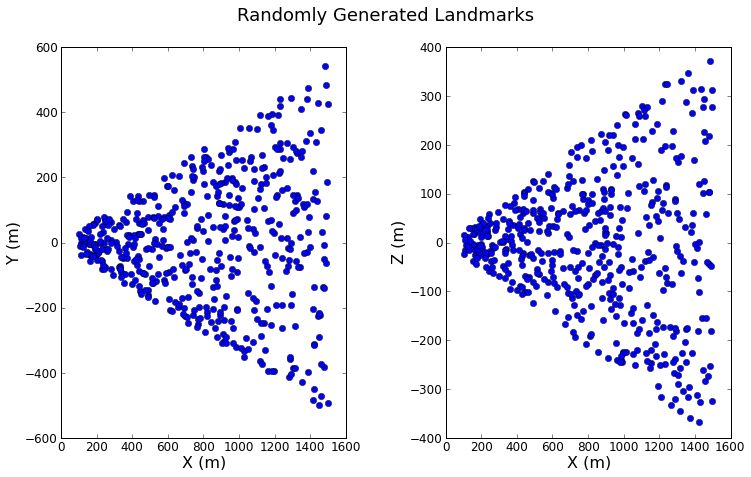
\includegraphics[width=12cm, height=7cm]{./Figures/SimulationFigures/Figure51.png}
\caption{Randomly Generated 3D Landmark Points}
\label{fig:simfig51}
\end{figure}
\FloatBarrier

\section{An Ideal Case}
% word checked.
First of all, understanding the algorithm's performance under nearly
no noise condition provides a solid ground for the analysis later on.
This simulation showed how much error the model itself generated under
the most basic flying condition, which is moving forward at constant
speed. The low noise environment was configure as such,

\begin{itemize}
  \item SUAS was moving forward (X axis) with constant speed at 60 knots. 
  \item Y axis and Z axis translation were limited to white noise with
  standard deviation of 0.08 meters and a mean of 0.
  \item SUAS rotation were modelled by white noise with standard
  deviation of 0.01 degree and a mean of 0
  \item No image digitization (i.e. the projected landmark position on
  image plane was not digitized to any sensor resolution)
  \item No error was introduced from camera model mismatch (i.e.
  camera model used by simulator is exactly the same as the one used
  by CC\_EKF\_SLAM algorithm.
\end{itemize}

\subsection{UAV Localization}
% word checked.
UAV poses were plotted in Figure \ref{fig:simfig1}. The ground truth
and estimated value are plotted in blue and green lines respectively.
The error defined by $Estimated-Ground Truth$ is plotted in red line.
Under a simple forward only motion, the algorithm tracked the UAS
status quite well, with error on translational motion less than 1 cm
and error on rotational motion less than 3e-3 degree.

\begin{figure}[h]
\centering
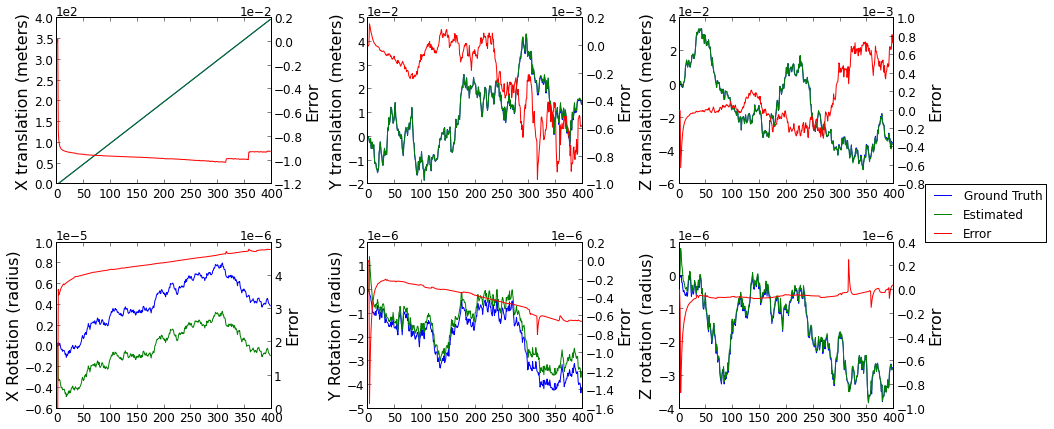
\includegraphics[width=15cm, height=7cm]{./Figures/SimulationFigures/Figure1.png}
\caption{UAS localization error under no noise condition}
\label{fig:simfig1}
\end{figure}
\FloatBarrier

\subsection{Landmarks Mapping - Convergence and Accuracy}
% word checked.
Figure \ref{fig:simfig5-8} top left shows landmark parameters $[d, \varphi ,\theta]$ (where $d=1/\rho $) plotted against frame number for the first 50 frames. The landmark depth $d$ for all landmarks converged within 3 frames; elevation-azimuth angles $[\varphi ,\theta]$ stay almost constant after initialization. A more detail graph can be seen from the error convergence plot for these parameters (Figure \ref{fig:simfig5-8} top right.) which shows the tracking error of these parameters for 400 frames. The error of landmark distance $d$ continues to approach zero as the tracking continues. $[\varphi ,\theta]$ show small drift within $+/-0.0002^{\circ}$ respectively. However, as tracking continue into later frames, error of $[\varphi ,\theta]$ gradually grew bigger. The resulting error for landmark coordinate in world frame represented in standard Euclidean XYZ parameterization are plotted against initialization sequence and frame number, and are shown in figure \ref{fig:simfig5-8} bottom left and right. The landmarks positions errors in world frame converge to zero as tracking continues. During the process, some landmarks moved out of the FOV, and therefore its position estimate remained unchanged since then. At the end of the 400 frames, the x axis position error of the landmark reduced to +/-0.2 meters; y and z axis error reduce to +/-0.02 meters

\begin{figure}[h]
\centering
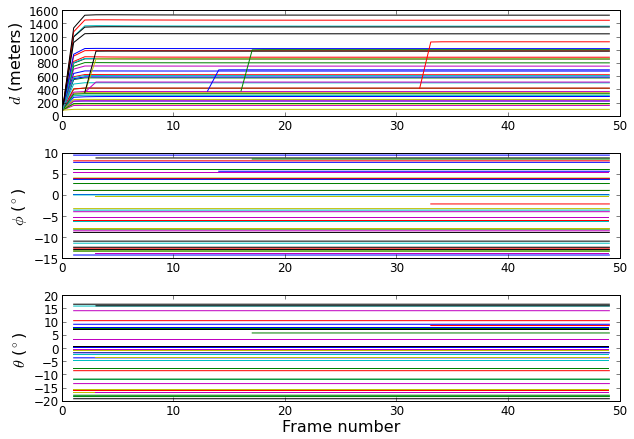
\includegraphics[width=7cm, height=5cm]{./Figures/SimulationFigures/Figure6.png}
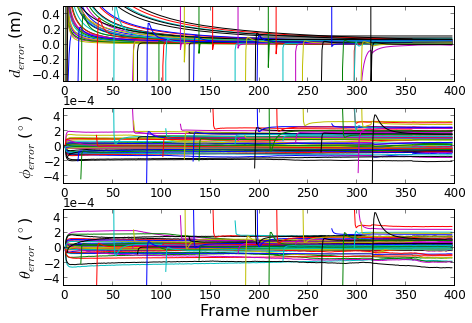
\includegraphics[width=7cm, height=5cm]{./Figures/SimulationFigures/Figure7.png}
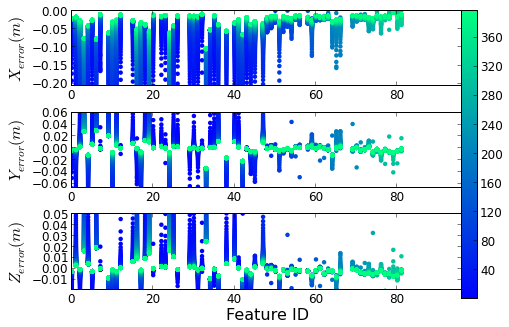
\includegraphics[width=7cm, height=5cm]{./Figures/SimulationFigures/Figure5.png}
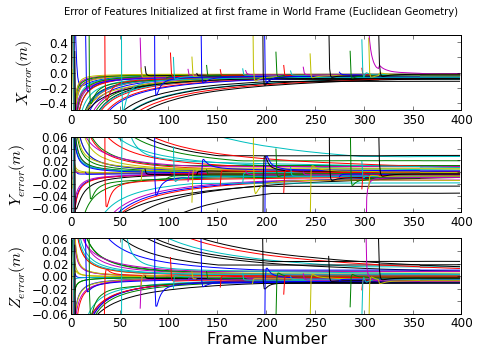
\includegraphics[width=7cm, height=5cm]{./Figures/SimulationFigures/Figure8.png}
\caption{Landmarks parameters and error convergence under low noise condition}
\label{fig:simfig5-8}
\end{figure}

\section{Effect of SUAS Motion}
% word checked. 
The simulation result from UAS forward travel shows that the CC\_EKF\_SLAM algorithm does landmark tracking and self localization quite well under simple SUAS motion. Next, the algorithm is tested with a more complex and realistic scenario. A series of motion is added to the simulation in addition to the forward motion. The remaining 5 types of maneuvers were added one at a time. These maneuvers are: translation on Y, translation on Z, rotation on X, rotation on Y and rotation on Z. Each motion is modelled by a sine wave with frequency at 1Hz, and variable amplitude. For translation simulations, the sine amplitude varies from 1 meter to 19 meters with 2 meters increments. For rotation simulations, the amplitude varies from 0.001 radius to 0.018 radius with 0.001 radius increment.

\subsection{SUAS Localization under Motion}

Figure \ref{fig:simfig9-10} shows the SUAS localization error statistic under translation motion on Y and Z axis and rotation motion on X, Y, and Z axis. The blue dots mark the mean value $\mu$ of the error throughout 400 frames of tracking, and the error bars mark the standard deviation $\sigma$.

The translation motion clearly increases the error of SUAS localization. However, the amount is insignificant. With the Sine amplitude increased to 19m, SUAS position error increased by less than 0.02 meter.

On the other hand, rotation motions have a big impact on the accuracy
of localization. Rotation on X axis (roll) has small effect on the accuracy of SUAS position and orientation estimate. No obvious increase on mean and standard deviation of the error can be observed. Rotations on Y and Z axis yield significant error.

\begin{itemize}
  \item Rotation on Y axis increases the SUAS X position mean error, as well as the standard deviation. For Z position of the SUAS, the mean error stays zero, but standard deviation increase dramatically.
  \item Same thing happens to the X and Y position for rotation on Z axis.
\end{itemize}

\begin{figure}[h]
  \centering
  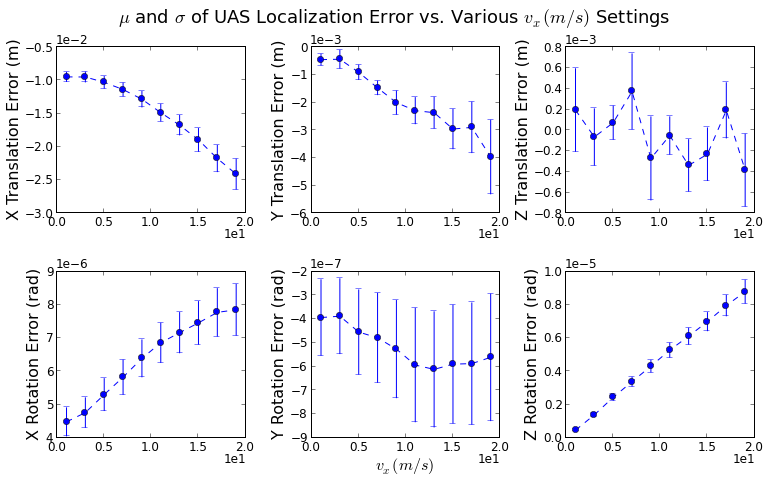
\includegraphics[width=4.5cm, keepaspectratio=true]{./Figures/SimulationFigures/Figure9.png}
  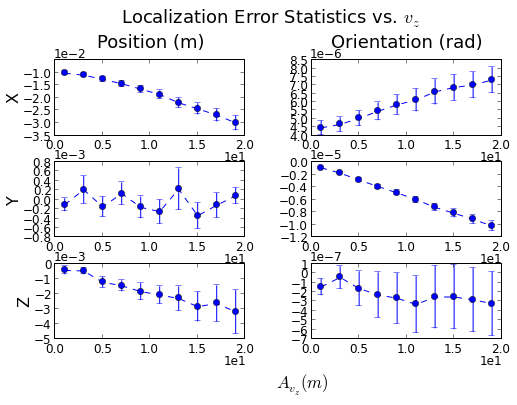
\includegraphics[width=4.5cm, keepaspectratio=true]{./Figures/SimulationFigures/Figure10.png}
  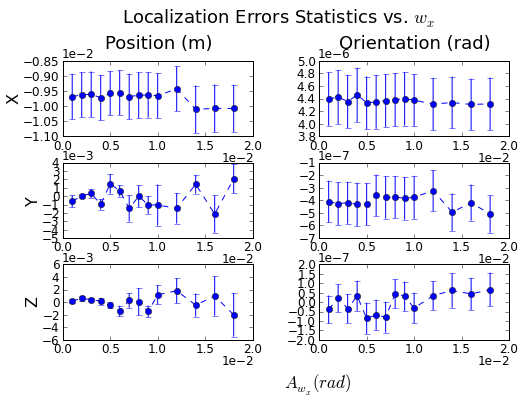
\includegraphics[width=4.5cm, keepaspectratio=true]{./Figures/SimulationFigures/Figure11.png}
  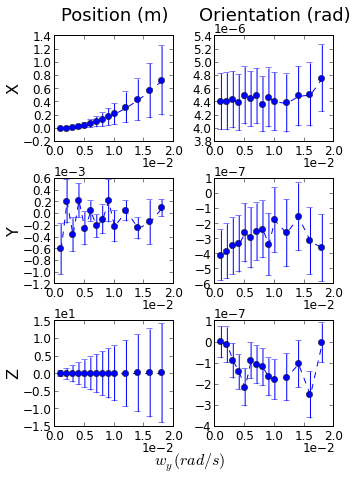
\includegraphics[width=4.5cm, keepaspectratio=true]{./Figures/SimulationFigures/Figure12.png}
  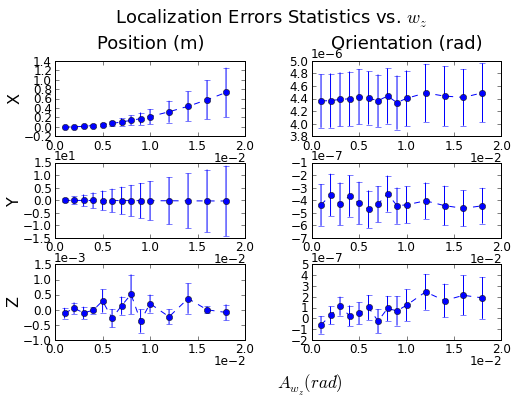
\includegraphics[width=4.5cm, keepaspectratio=true]{./Figures/SimulationFigures/Figure13.png}
  \caption{UAS localization error under translational 
  \label{fig:simfig9-10}
    motion}
\end{figure}
%\FloatBarrier

To understand how rotation motion affect the SUAS localization estimate, the SUAS position on X, Y, Z in world frame are plotted below (figure \ref{fig:simfig14}) with rotation amplitude on X, Y and Z set at 0.01 radius. When rotation occurred on X axis, the position error of SUAS shows some oscillation. The oscillation magnitude remains small (in the scale of millimeters) and around zero. For rotation on Y and Z, the situation is very different. Both rotation motions caused the SUAS position error to oscillate with the oscillation amplitude increasing (diverging) as tracking goes on. The X position error of the SUAS increases in positive value with rotation occurring on Y and Z, but the most significant impact happens on the Z position (for rotation on Y) and Y position (for rotation on Z), with error reaching 20 meters peak-to-peak at the end of the 400 frames. With increasing rotation rate (amplitude of the sine wave), the rate of error diverging from zero also increases, hence, resulting in an increasing error standard deviation in error statistic plots. This simulation result suggests that CC\_EKF\_SLAM algorithm is very sensitive to rotation on Y and Z axis.

\begin{figure}[h]
  \centering
  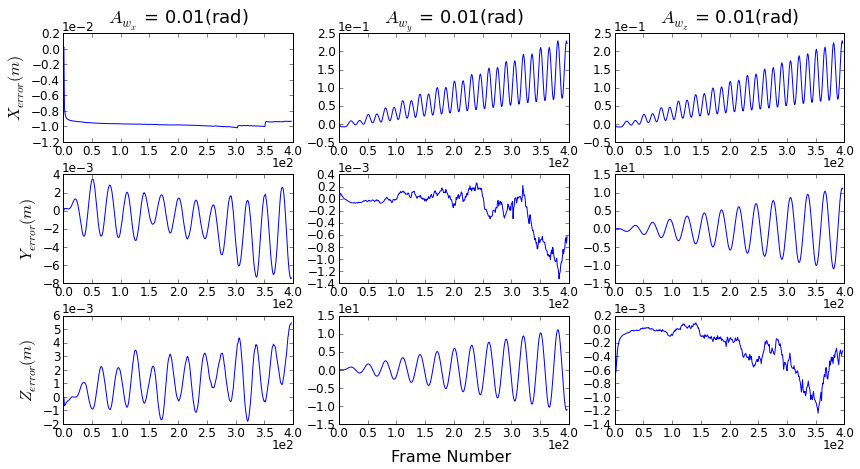
\includegraphics[width=13cm, keepaspectratio=true]{./Figures/SimulationFigures/Figure14.png}
  \caption{UAS estimated position in world frame}
  \label{fig:simfig14}
\end{figure}
\FloatBarrier
\subsection{Landmark Mapping Accuracy under Motion}\label{sec:landmarkMotion}
% word checked.
Landmark mapping error statistic are calculated from the landmark error at last frame, since landmarks error converge to zero as tracking goes on. Figure \ref{fig:simfig20-24} shows the landmark mapping error statistic with added motions. Translation motions increase both the error mean and standard deviation, but not by much. With the motion maximum amplitude ranging from 1 meter to 19 meters, the increases of landmarks position error mean and standard deviation are both in the scale of centimeters.

\begin{figure}[h]
  \centering
  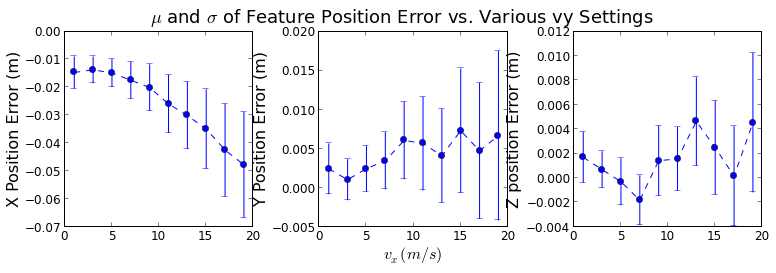
\includegraphics[width=7cm, height=2.5cm]{./Figures/SimulationFigures/Figure20.png}
  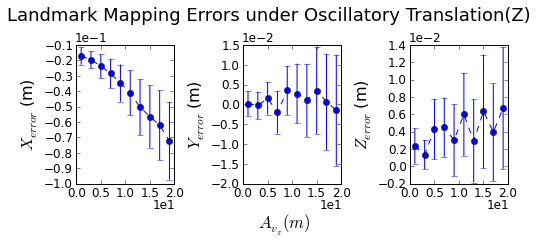
\includegraphics[width=7cm, height=2.5cm]{./Figures/SimulationFigures/Figure21.png}
  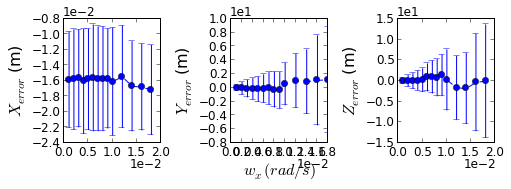
\includegraphics[width=7cm, height=2.5cm]{./Figures/SimulationFigures/Figure22.png}
  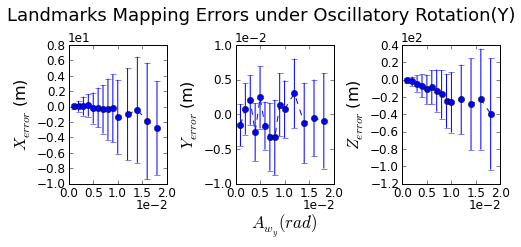
\includegraphics[width=7cm, height=2.5cm]{./Figures/SimulationFigures/Figure23.png}
  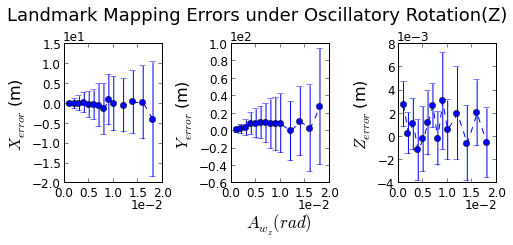
\includegraphics[width=7cm, height=2.5cm]{./Figures/SimulationFigures/Figure24.png}
  \caption{Landmark mapping error under added motion}
  \label{fig:simfig20-24}
\end{figure}

With maximum rate of rotation ranging from 0.001 radius/frame to 0.018
radius/frame

\begin{itemize}
  \item Rotations on all three axis yield significant error increase for landmark position estimate,
  \item X axis rotation causes increase on standard deviation on Y and Z axis by similar amount. The errors are in the scale of meters with maximum rotation setting.
  \item Y axis rotation causes increase on mean and standard deviation on X and Z axis. Z axis landmark position receives the biggest impact with error in the scale of hundreds of meters with maximum rotation setting
  \item Z axis rotation impacts on X and Y axis landmark position in a
  similar way as the Y axis rotation does.
\end{itemize}

\begin{figure}[h]%redo plots
  \centering
  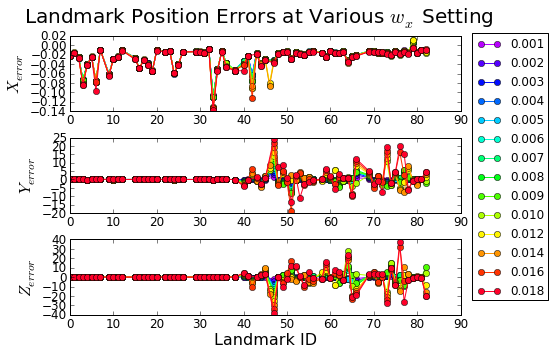
\includegraphics[width=7cm, height=5cm]{./Figures/SimulationFigures/Figure17.png}
  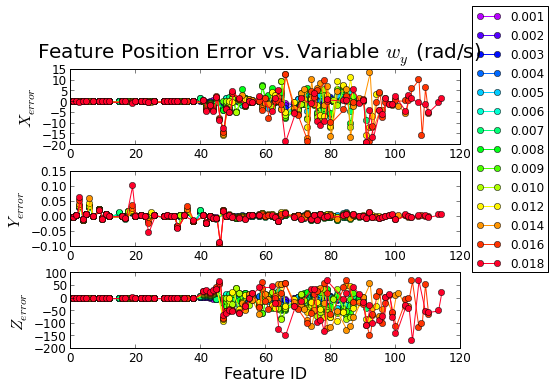
\includegraphics[width=7cm, height=5cm]{./Figures/SimulationFigures/Figure18.png}
  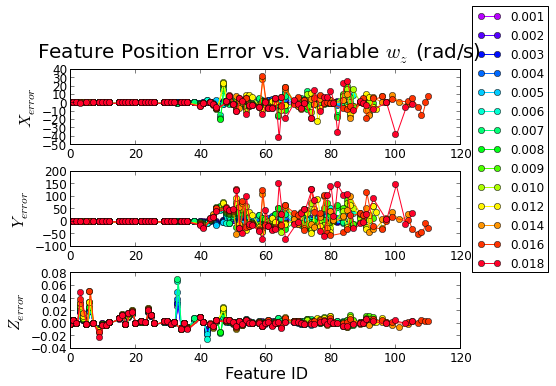
\includegraphics[width=7cm, height=5cm]{./Figures/SimulationFigures/Figure19.png}
  \caption{Landmark mapping error under rotational motion}
  \label{fig:simfig17-19}
\end{figure}

Figure \ref{fig:simfig17-19} shows the landmarks position error at the last tracking frame plotted against initialization sequence, with line and marker color indicating various rotation amplitude setting.

\begin{itemize}
  \item With rotation on Y and Z, the tracked landmarks easily went out of FOV. This can be observed from total number of landmarks went from 80 to over 110 with Y axis rotation setting varied from 0.001rad/s to 0.018rad/s. This caused frequent additions of new landmarks.
  \item Landmarks added after first frame has much bigger error than landmarks added at first frame. At 1$^{st}$ frame, 40 landmarks were added to the filter. Error plots from Y and Z axis rotation both shows that major landmark mapping error came from landmarks added after the 1 $^{st}$ frame with ID bigger than 40.
\end{itemize}
\FloatBarrier

To investigate how does rotation motion results in bigger error on landmarks added after first frame, landmarks parameters error (after being converted to world frame) with $w_y = 0.01$ are plotted in figure \ref{fig:simfig25}. It is found that the most significant error happen to parameter $\varphi$ which is the landmark elevation angle. This angle has the same definition as rotation angle around Y axis. The second contributor is $z_i$, the Z axis coordinate of the landmark initialization point. Both parameters have an offset error at initialization, and were never corrected throughout the tracking.

Figure \ref{fig:simfig26} shows the $\varphi$ error at initialization in camera frame and world frame. The blue line shows the error in camera frame. The red line shows the error in world frame transformed using the estimated UAS position and orientation. It is clear that it is the transformation process that introduced the offset error in $\varphi$. Offset error in $z_i$ is due to the same reason. As the result from previous section indicated, with Y axis rotation, SUAS localization estimate has the biggest error in position on X and Z axis. In addition, ground truth landmarks were transformed using the ground truth SUAS position and orientation, which is different than the estimated ones. It is not surprised that the transformation process introduced offset error into the landmark parameters. Landmarks initialized at first frame don't carry any offset error because the transformation process is using the same parameters in both way. During tracking, these landmarks are transformed to the new camera frame using the estimated SUAS position and orientation. These are the same estimation being used to transform landmark position from camera frame back into world frame. Therefore, although the SUAS localization estimations are different from the ground truth, landmark initialized at first frame were not affected. To conclude, the major contributor for landmark mapping error came from error in UAS localization estimation.

\begin{figure}[h]
  \centering
  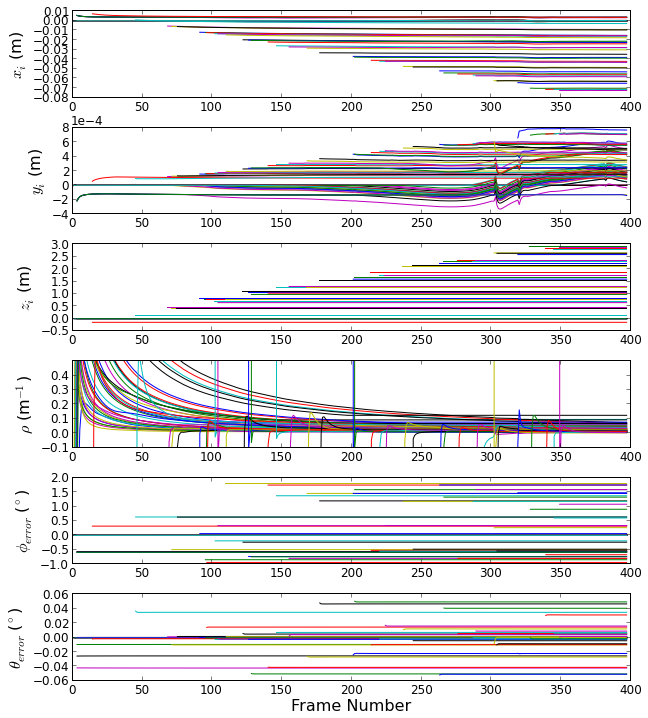
\includegraphics[width=10cm, height=12cm]{./Figures/SimulationFigures/Figure25.png}
  \caption{Landmark parameters error under rotational motion}
  \label{fig:simfig25}
\end{figure}

\begin{figure}[h] %redo figure, change phi to varphi
  \centering
  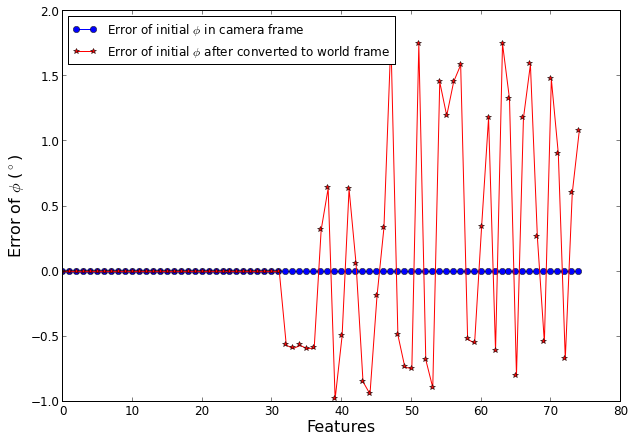
\includegraphics[width=10cm, height=7cm]{./Figures/SimulationFigures/Figure26.png}
  \caption{Error of $\varphi$ in camera frame and world frame at initialization}
  \label{fig:simfig26}
\end{figure}
\FloatBarrier

\section{Camera Intrinsic Parameters}
% word checked.
This section summarizes the impact of inaccurate camera parameters estimates. Error on camera intrinsic parameters is simulated by using different values in the camera models used by the simulator and the CC\_EKF\_SLAM algorithm. $c_{x}$, $c_{y}$, $f_{x}$, and $f_{y}$ are simulated individually and distortion parameters $[k1, k2, p1, p2]$ are simulated as a group. Using the calibrated camera model (see section \ref{sec:camcal}) as a base model,$ c_{x}$, $c_{y}$, $f_{x} $, and $f_{y}$ in simulator camera model varied from -50\% to 50\% of the base model. Distortion parameters varied from 0\% to 140\% of the base model.

\subsection{Effect from $(c_{x}, c_{y})$}
% word checked.
Figure \ref{fig:simfig34-35} show an overview of SUAS localization error statistics with incorrect estimates of $ (c_{x}, c_{y})$. From the statistic plot, it is found that $c_x$ has impact on SUAS position on X and Y, while $c_y$ has impact on SUAS position on X and Z. 

\begin{figure}[h]
  \centering
  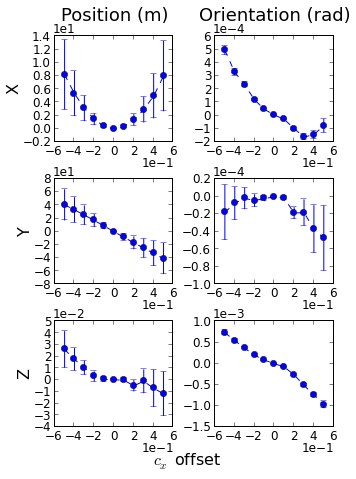
\includegraphics[width=5cm, keepaspectratio=true]{./Figures/SimulationFigures/Figure34.png}
  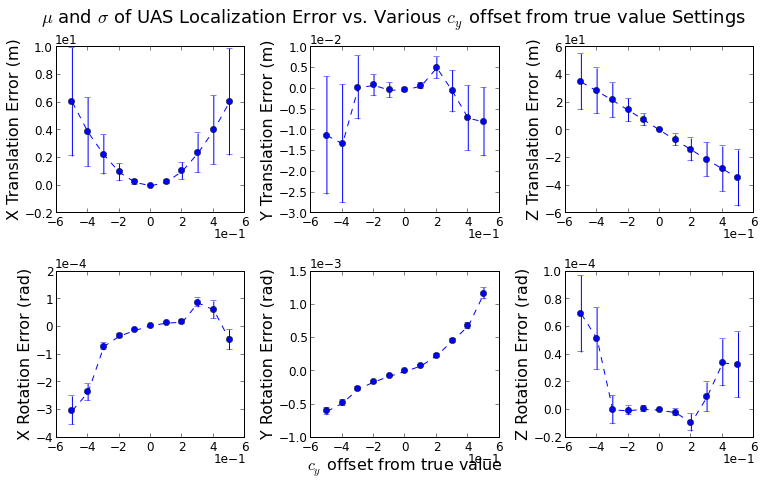
\includegraphics[width=5cm, keepaspectratio=true]{./Figures/SimulationFigures/Figure35.png}
  \caption{SUAS localization error statistic with varying $(c_x, c_y)$}
  \label{fig:simfig34-35}
\end{figure}

Figure \ref{fig:simfig36-37} shows the SUAS position error with various $c_x$ and $c_y$. SUAS position error is dependent on both $(c_{x}, c_{y})$ and time. The SUAS position error is diverging (increasing in time), and can be modeled by 1 $^{st}$ order polynomial function, with the rate of diverging decided by the error of $(c_{x}, c_{y})$. 

\begin{figure}[h]
  \centering
  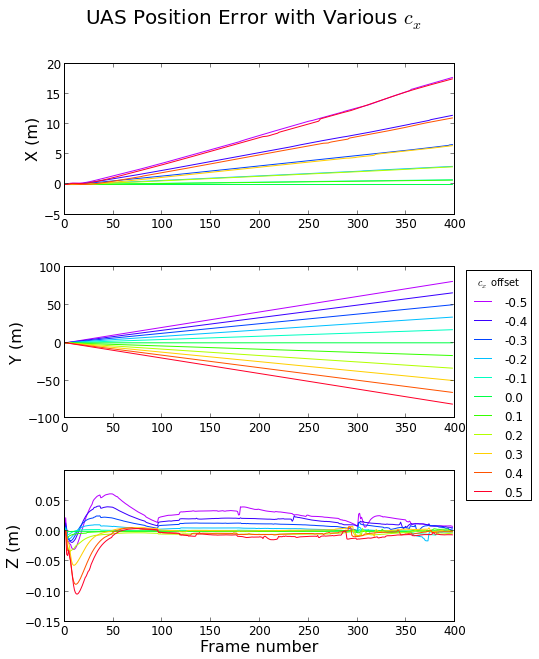
\includegraphics[width=7cm,keepaspectratio=true]{./Figures/SimulationFigures/Figure36.png}
  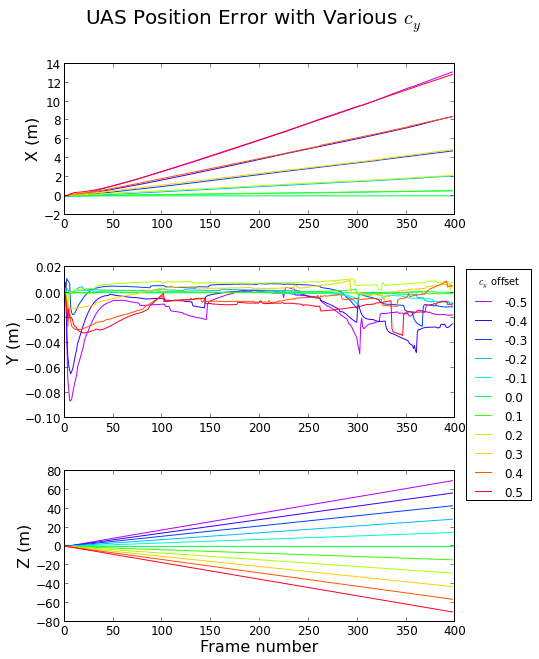
\includegraphics[width=7cm,keepaspectratio=true]{./Figures/SimulationFigures/Figure37.png}
  \caption{Diverging SUAS position error}
  \label{fig:simfig36-37}
\end{figure}
\FloatBarrier

The landmark mapping error statistics from incorrect estimate of $ (c_{x}, c_{y})$ are plotted in figure \ref{fig:simfig28-29}. The following characters can be observed from the plots:

\begin{itemize}
  \item Incorrect $c_{x}$ affect landmark position on all axis, among which, X and Y axis see the most significant error.
  \begin{itemize}
    \item The further $c_{x}$ deviate from the true value, the further the landmarks appear (positive X axis error).
    \item On Y axis, inaccurate $c_x$ causes offset error in landmark position. 
    \item Incorrect $c_{x}$ also affect Z axis landmark position, but by a much smaller amount.
  \end{itemize}
  \item Incorrect $c_{y}$ affect landmark position on all axis similarly to $c_{x}$. Estimates on X and Z axis show most amount of error.
\end{itemize}

\begin{figure}[h]
  \centering
  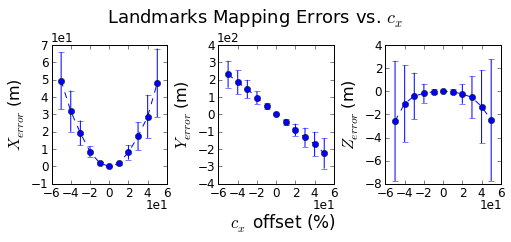
\includegraphics[width=7cm, keepaspectratio=true]{./Figures/SimulationFigures/Figure28.png}
  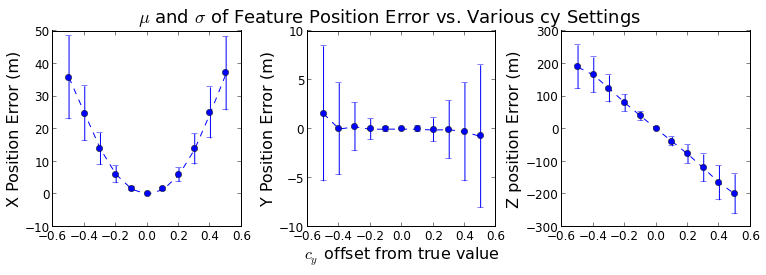
\includegraphics[width=7cm, keepaspectratio=true]{./Figures/SimulationFigures/Figure29.png}
  \caption{Landmark mapping error statistic with varying $(c_x, c_y)$}
  \label{fig:simfig28-29}
\end{figure}

Plotting landmark position error as a function of landmarks ground truth positions reveals more information on how incorrect $c_{x}$ and $c_{y}$ affect landmark mapping. Landmark position error is a function of its ground truth position, and $c_{x}$ (or $c_{y}$).

\begin{itemize}
  \item Landmark position error on X axis is proportional to the landmark ground truth position on X. The further the landmark is, greater the error will be. The degree of incorrectness in $c_{x}$ decide the slope of the error plot, greater the error in $c_{x}$, steeper the slope (figure \ref{fig:simfig32-33} left, subplot $[1,1]$).
  \item Landmark position error on Y axis is also proportional to it's ground truth position on X with the slope polarity dependable on the polarity of the error of $c_{x}$, and slope dependable on the error on $c_{x}$ (figure \ref{fig:simfig32-33} left, subplot $[2,1]$).
  \item Landmark position error on Z axis is proportional to its ground truth position on Z, with slope polarity dependable on the polarity of error of $c_{x}$, and slope dependable on the error of $c_{x}$ (figure \ref{fig:simfig32-33} left, subplot $[3,3]$).
\end{itemize}

$c_{y}$ affects landmark position similarly to $c_{x}$ (figure \ref{fig:simfig32-33}, right).

\begin{figure}[h]
  \centering
  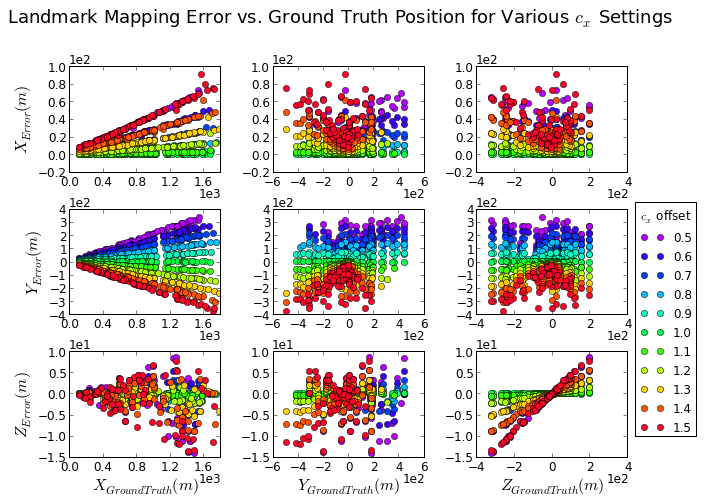
\includegraphics[width=7cm, height=5cm]{./Figures/SimulationFigures/Figure32.png}
  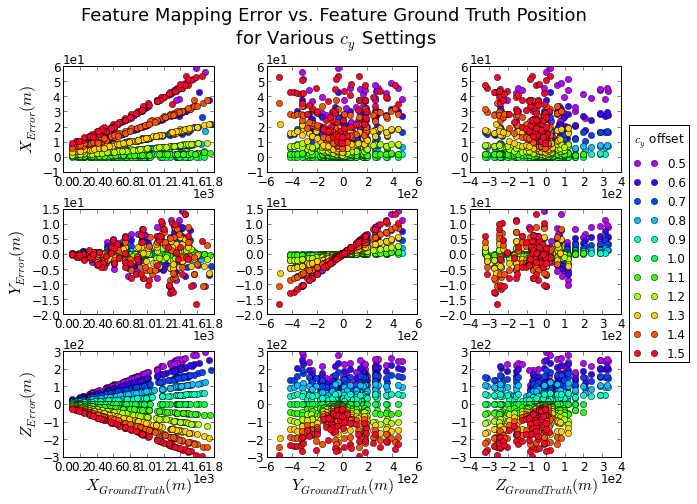
\includegraphics[width=7cm, height=5cm]{./Figures/SimulationFigures/Figure33.png}
  \caption{Landmark mapping error vs. ground truth landmark position}
  \label{fig:simfig32-33}
\end{figure}
\FloatBarrier

\subsection{Effect from $(f_x, f_y)$}

With $(f_x, f_y)$ varying from -50\% to +50\% of the calibrated value, the SUAS localization error is shown in \ref{fig:simfig43-44}. For all $f_x$ and $f_y$ settings, SUAS position error remained less than +/-0.05 meters, and orientation error remained in less than 8e-6 radius. Compared to the error obtained from the ideal case simulation, Error in $(f_x, f_y)$ does not introduce any additional error into SUAS localization estimate. 
\begin{figure}[h]
  \centering
  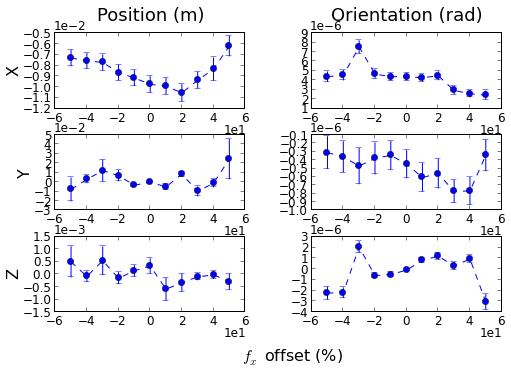
\includegraphics[width=5cm,keepaspectratio=true]{./Figures/SimulationFigures/Figure43.png}
  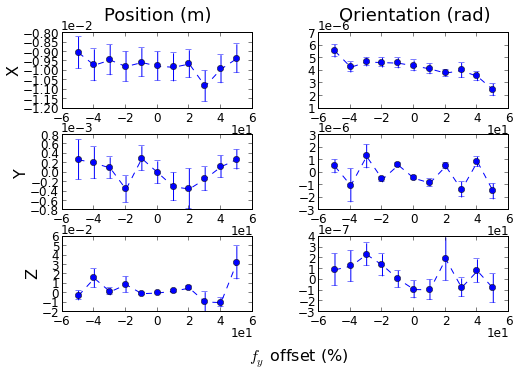
\includegraphics[width=5cm,keepaspectratio=true]{./Figures/SimulationFigures/Figure44.png}
  \caption{UAS localization error statistic with variable $(f_x, f_y)$}
  \label{fig:simfig43-44}
\end{figure}

Landmark mapping, on the other hand, is unavoidably affected by the
error in $(f_x, f_y)$ since these are the scaling factor that project
landmarks from 3D world onto image plane. Figure \ref{fig:simfig38-39}
shows the error statistic of landmark position estimates under various
$(f_x, f_y)$ settings. The effect on the X axis component is minimal
and is in the scale of millimeter. Y axis component receive the most
impact with inaccurate $f_x$, since this is the scale factor that map
landmark's Y component in world frame onto U axis on image plane by $u
= Y/X \cdot f_x$. Same behavior happens for the Z axis component of
the landmark position estimate and its relation to $f_y$.

\begin{figure}[h]
  \centering
  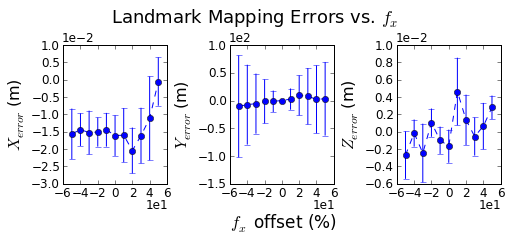
\includegraphics[width=7cm,keepaspectratio=true]{./Figures/SimulationFigures/Figure38.png}
  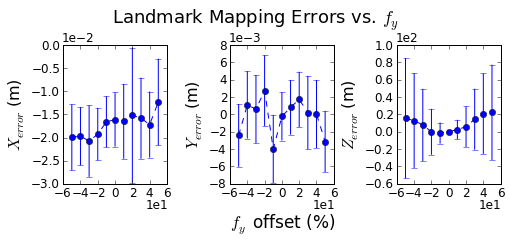
\includegraphics[width=7cm,keepaspectratio=true]{./Figures/SimulationFigures/Figure39.png}
  \caption{Landmark mapping error statistic with variable $(f_x, f_y)$}
  \label{fig:simfig38-39}
\end{figure}

Plotting the landmark mapping error against landmark ground truth position reveals how error in $(f_x, f_y)$ impact on landmark position estimates. When $f_x$ contains error, Y component of landmark position error is directly proportional to the Y component of its ground truth position, with the error in $f_x$ determines the function's slope. Same relation can be found for $Z_{error}$ with $f_y$, and $Z_{ground truth}$.

\begin{figure}[h]
  \centering
  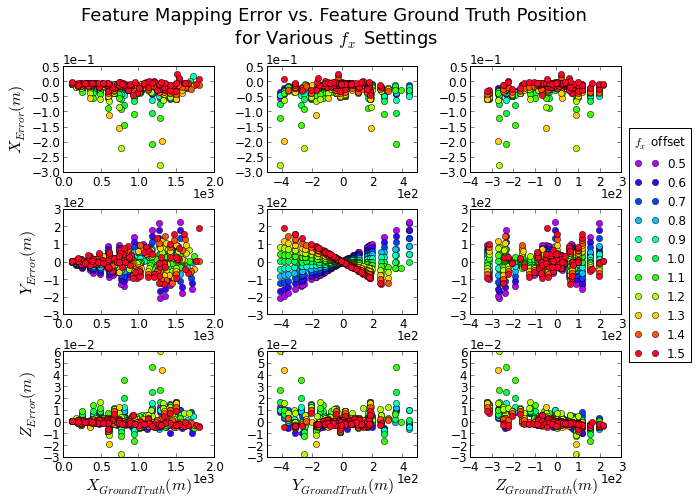
\includegraphics[width=7cm,keepaspectratio=true]{./Figures/SimulationFigures/Figure41.png}
  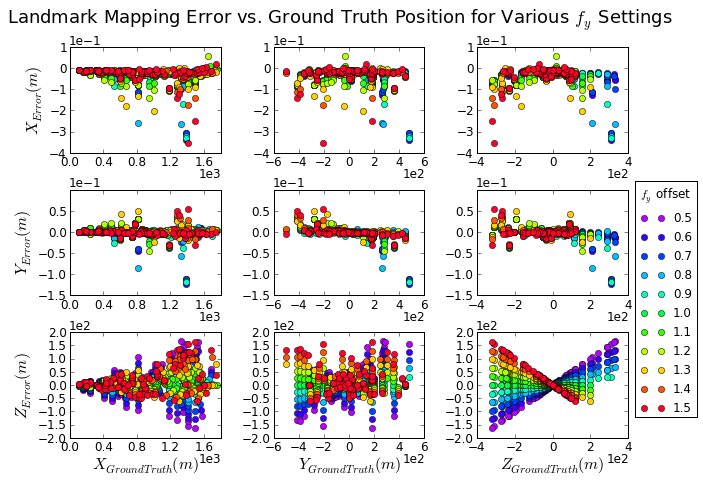
\includegraphics[width=7cm,keepaspectratio=true]{./Figures/SimulationFigures/Figure42.png}
  \caption{Landmark mapping error plotted against landmark ground truth
    for various $(f_x, f_y)$}
  \label{fig:simfig38-39}
\end{figure}

\FloatBarrier

\subsection{Effect from Distortion}
% word checked.
The CC\_EKF\_SLAM algorithm does not consider camera lens distortion at this stage. Therefore, the simulation evaluate the effect of distortion varying from 0\% to 150\% of the calibrated result to evaluate the amount error resulted by ignoring the lens distortion. 

Figure \ref{fig:simfig48} (left) shows the SUAS localization error for all lens distortion setting. Ignoring the distortion brings significant error into the UAS localization. SUAS X position receives the most impact with error up to 100 meters with increasing standard deviation. Y and Z position shows less error, but standard deviation grows larger with the increase in distortion offset. Figure \ref{fig:simfig48} (right) reveals the cause of increasing standard deviation. The SUAS position error was diverging with time. The SUAS orientation error increased from maximum mean error of 5e-6 radius in low noise simulation to 2.5e-4 rad. The standard deviation of orientation estimates also increased with lens distortion offset. Similarly, the plots of orientation error vs. frame number show that the error amplitude increases with time, although it fluctuates around zero.

%TODO regenerate figure to make X axis more readable. change UAS to SUAS
\begin{figure}[h]
  \centering
  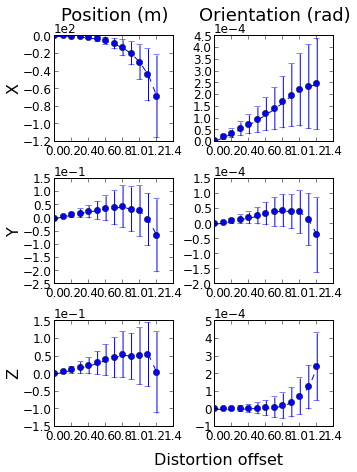
\includegraphics[width=5cm,keepaspectratio=true]{./Figures/SimulationFigures/Figure47.png}
  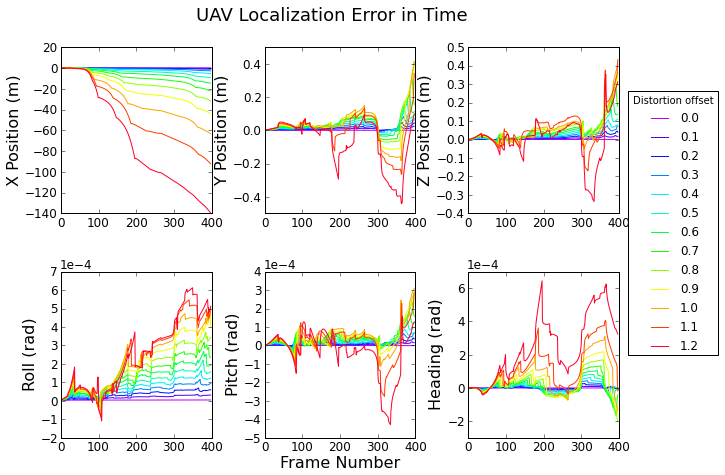
\includegraphics[width=9cm,keepaspectratio=true]{./Figures/SimulationFigures/Figure48.png}
  \caption{SUAS localization error with lens distortion}
  \label{fig:simfig48}
\end{figure}

The landmark position error statistic is shown in figure \ref{fig:simfig45}. The X axis of landmark position shows the most error, with mean value reading -400 meters with distortion offset at 150\%. Y, and Z axis position has less mean error, but the standard deviation is bigger. Plotting landmark position error against landmark ground truth coordinate (figure \ref{fig:simfig46}) shows that the increasing standard deviation is due to the first order linear relation between the Y (or Z) axis of landmark position error and the Y (or Z) axis of landmark ground truth coordinate, where distortion offset determine the slope of the line. The relation indicates that landmark lying around the sides of the image plane carries more error than landmarks at the center of the image. This is exactly the kind of error that radial distortion corrects for. 

\begin{figure}[h]
  \centering
  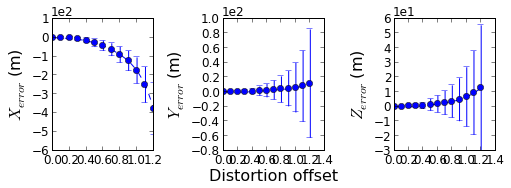
\includegraphics[width=10cm,keepaspectratio=true]{./Figures/SimulationFigures/Figure45.png}
  \caption{Feather position error with lens distortion}
  \label{fig:simfig45}
\end{figure}

\begin{figure}[h]
  \centering
  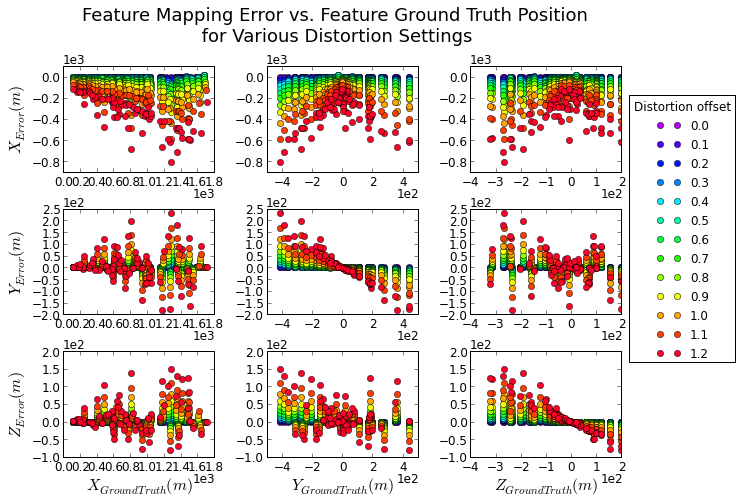
\includegraphics[width=10cm,keepaspectratio=true]{./Figures/SimulationFigures/Figure46.png}
  \caption{Feather position error vs. ground truth position with lens distortion}
  \label{fig:simfig46}
\end{figure}

\FloatBarrier

\subsection{Effect from Image Resolution}

It is well known that higher resolution sensor will give more accuracy to the estimate. To know how high a resolution is good enough for the distance range that this research is targeting at, a quantitative analysis is necessary. A few simulation is ran with various image resolution settings, and the result is shown in figure \ref{fig:simfig50}. 

%TODO regenerate top figure to give enough room for xlabel, change UAS
%to SUAS
\begin{figure}[h] 
  \centering
  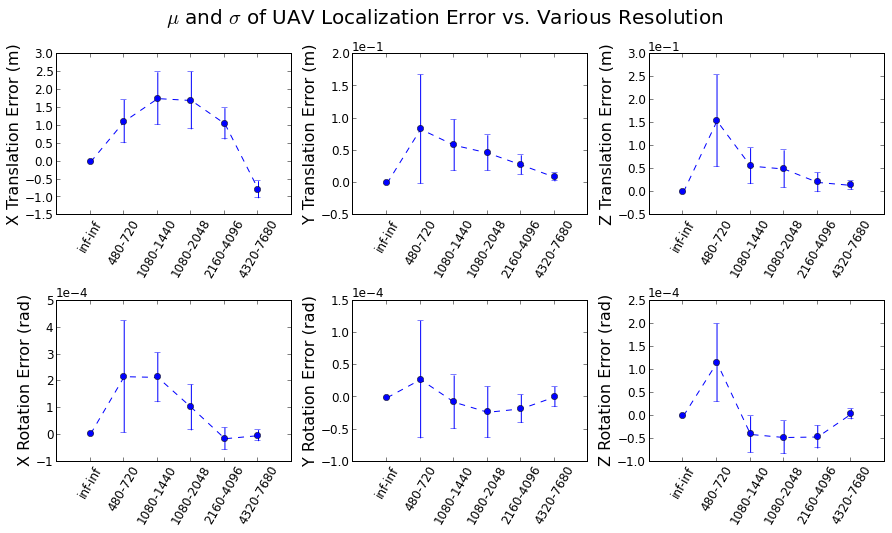
\includegraphics[width=10cm,keepaspectratio=true]{./Figures/SimulationFigures/Figure50.png}
  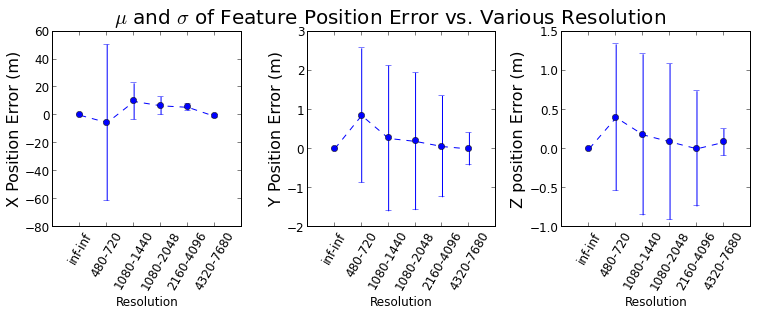
\includegraphics[width=10cm,keepaspectratio=true]{./Figures/SimulationFigures/Figure49.png}
  \caption{Error statistic for various image resolution}
  \label{fig:simfig50}
\end{figure}

This test confirmed that the higher resolution the image sensor is, the more accuracy it will bring. The most significant error is seen at resolution 480x720 where the X axis of landmark position error is +/- 150m. At 720x1080, which is one step up of 480x720, the X axis landmark position error is greatly reduced to a few meters. For all other parameters, improvement at each level of resolution increase is nearly linear. This result suggests that to achieve reasonably good accuracy for obstacle detection, a resolution of 720x1080 or higher is preferred. 


%%% Local Variables:
%%% mode: latex
%%% TeX-master: "thesis"
%%% End:
